\section{Вход в АРМ вуза} \label{sec:cabinet}
Для входа в АРМ вуза необходимо нажать на значок \quotes{Мой профиль} в верхнем правом углу страницы (рис.~\ref{img:university_select:icon}),
после чего на экране появится список доступных действий.

\begin{figure}[H]
	\center{
\includegraphics[width=0.4\linewidth]{images/university_select/icon}}
	\caption{Значок \quotes{Мой профиль}}
	\label{img:university_select:icon}
\end{figure}
Если количество доступных пользователю АРМ вузов от одного до трёх, в меню будут отображены названия всех этих вузов (рис.~\ref{img:university_select:select_university_less_3}). При нажатии на любой из перечисленных в меню вузов откроется страница АРМ соответствующего вуза.

\begin{figure}[H]
	\center{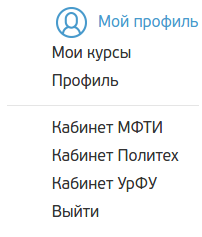
\includegraphics[width=0.4\linewidth]{images/university_select/select_university_less_3}}
	\caption{Внешний вид меню с тремя доступными вузами}
	\label{img:university_select:select_university_less_3}
\end{figure}

Если количество доступных пользователю АРМ вузов больше трёх, в меню будет отображен пункт \quotes{Кабинеты вузов} (рис.~\ref{img:university_select:select_university_more_3})

\begin{figure}[H]
	\center{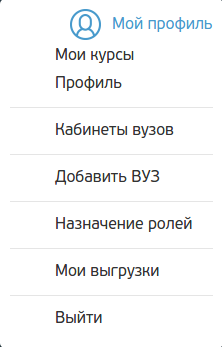
\includegraphics[width=0.4\linewidth]{images/university_select/select_university_more_3}}
	\caption{Внешний вид меню при количестве вузов более трёх}
	\label{img:university_select:select_university_more_3}
\end{figure}

При выборе данного пункта меню на экране появится окно, в котором необходимо выбрать вуз из списка (работа со списком подробно описана в пункте~\ref{widget:autocomplete}) и нажать на кнопку \vcenteredinclude[height=25px]{images/university_select/university_select_btn}, после чего пользователь будет перенаправлен в АРМ соответствующего вуза.
\begin{figure}[H]
	\center{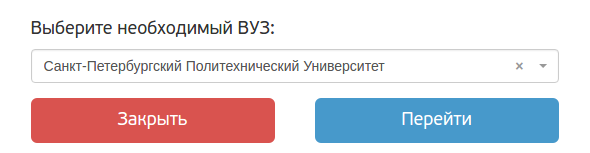
\includegraphics[width=1\linewidth]{images/university_select/select_university_dialog}}
	\caption{Окно выбора вуза}
	\label{img:university_select:select_university_dialog}
\end{figure}

Для того, что бы закрыть данный диалог, необходимо нажать на кнопку \vcenteredinclude[height=25px]{images/university_select/university_select_close_btn} или кликнуть на область вне диалога.